\documentclass[letterpaper]{article}
\usepackage{aaai}
\usepackage{times}
\usepackage{helvet}
\usepackage{courier}
\usepackage{amsmath,amsfonts,amssymb,amsthm}
\usepackage{array}
\usepackage{amsmath,amssymb}
\usepackage{epsfig,subfigure}
\usepackage[vlined,algoruled,titlenumbered,noend]{algorithm2e}
\frenchspacing

\newcommand{\MarsRover}{\textsc{Mars Rover}}
\newcommand{\MarsRoverL}{\textsc{Mars Rover Linear}}
\newcommand{\MarsRoverNL}{\textsc{Mars Rover Nonlinear}}
\newcommand{\InventoryControl}{\textsc{Inventory Control}}
\newcommand{\WaterReservoir}{\textsc{Water Reservoir}}
\newcommand{\MultiWaterReservoir}{\textsc{Multi-Reservoir}}
\newtheorem*{example*}{Example}

\setcounter{secnumdepth}{0}  

 \begin{document}
% The file aaai.sty is the style file for AAAI Press 
% proceedings, working notes, and technical reports.
%
\title{Symbolic Dynamic Programming for Continuous action MDPs}
\author{Zahra Zamani\\
NICTA \& the ANU\\
Canberra, Australia\\
{\tt zahra.zamani@anu.edu.au}
\And
Scott Sanner\\
NICTA \& the ANU\\
Canberra, Australia\\
{\tt ssanner@nicta.com.au}
\And
Cheng Feng\\
Department of Aeronautics and\\
Astronautics, MIT, USA\\
{\tt cfang@mit.edu}
}
\maketitle
\begin{abstract}
\begin{quote}
Many real-world decision-theoretic problems require continuous actions as well as continuous 
states in order to plan optimally. While previous work has used methods such as discretization or 
sampling to approximately solve such problems, no exact solution has been introduced for both 
continuous state and action spaces. In this work, we take a symbolic approach to modelling domain 
problems with discrete and continuous state and action Markov decision processes (MDPs) and 
propose a symbolic dynamic programming solution to obtain the optimal policy. Crucially we show 
how that continuous maximization step in the dynamic programming backup can be evaluated 
optimally and symbolically; further we extend this maximization operation to work with an 
efficient and compact data structure, the extended algebraic decision diagram (XADD). We 
demonstrate empirical results for continuous state and action MDPs on a range of domains from 
planning and operations research to demonstrate the first exact optimal solution to these 
problems.
\end{quote}
\end{abstract}


\section{Introduction}


Markov decision processes (MDPs) have been a theoretical model for many planning problems in the recent years. Although the most common solution to MDPs is to use value iteration or policy iteration, they can quickly fall into Bellman's curse of dimensionality problem for large state – action spaces ~\cite{puterman}. In many problems this can be avoided by modelling the problem with continuous state – action spaces which is also a closer resemblance to real-world problems. 

Examples of problems in the continuous state and action domain can include Robotics, Operation Research and Management problems. The OR (Operation Research) literature has used MDPs to model many problems such as Inventory Control [] or Water Reservoir management []. These are examples where the state space can be modelled by discrete and continuous Markov decision processes and where the actions can also be considered continuous.

Most existing solutions concentrate on approximation techniques such as sampling [] that requires computational effort while providing no guarantee to the optimal solution, or other methods such as discretizing the state-action space[] that has scalability problems for large domain sizes. Meanwhile little effort has been devoted to exact solutions using the continuous variables beyond the piecewise rectilinear value function setting which contributes to a small subset of the problems in this domain. \\
In the previous paper [], the solution to continuous state MDPs was investigated, here we introduce a new model for Discrete and continuous state and Action MDPs (DCA-MDPs) and propose a new algorithm for value iteration in a Symbolic Dynamic Programming(SDP) format. Although the exact solution presented in [] covers the discrete and continuous state domain, it could not be used for planning in continuous action spaces. 

We exploit the algebraic properties of the maximization operator for continuous actions and develop disjoint case partitions that can be used to factor the actions in the Q-value to obtain the next value function. This symbolic maximization approach allows us to go beyond the linear function domain and apply the technique for non-linear reward and transition functions. Our method is scalable to higher horizons as well as being applicable to multi-variate continuous action domains. We represent the reward function as the function that is used to reward and penalize the agent based on the action costs. Both the reward and the transition function are represented using First-order logic with arbitrary piecewise symbol functions. These will be explained more deeply in section 2. This section also explains the main technique for applying continuous actions to any arbitrary function in depth. 

% Do we need any specific mention for the UB,LB, root of action here? 
The practical implementation of case statements of section 2 is the extended ADDs (XADDs) structure, which is discussed in section 3. In section 4 the symbolic value iteration algorithm for continuous action selection is presented and the approach of maximizing the action variables is examined by visual examples. Empirical results on various problems such as the Mars Rover, Inventory control and Water reservoirs are then demonstrated in section 5. We present some of the related works in section 6 and conclude with a discussion on the future work in the last section. 

\section{Case Representation}

To work in the symbolic space with lifted solutions, we need a representation for the symbolic functions and logical operators. Here we define such a notation along with the required operations for the SDP algorithm in the next sections. We consider the following simple example adopted from [] that is used throughout this paper:

\begin{example*}
[\MarsRoverNL] In a general \MarsRover\ domain, a rover is supposed to approach one or more target points and take images of these points.We consider the continuous non-linear example where the coordinate of the rover is a continuous variable $x$ and the amount of movement is also a continuous action $a$. A boolean variable $b$ is used for indicating whether the rover has already taken a picture at that point. The rover will move from any distance towards the target position of taking a picture only limited by the speed of moving. This constraints the rover to move more than 10 steps at a time. We consider the \MarsRoverNL  to have a non-linear transition or reward function.

\end{example*}

The \textit{case} notation can present any symbolic function in the following format: 

\begin{equation}
f = 
\begin{cases}
  \phi_1: & f_1 \\ 
 \vdots&\vdots\\ 
  \phi_k: & f_k \\ 
\end{cases}
\end{equation}

Where the $\phi_i$ are logical formulae defined over the state and action space $(\vec{b},\vec{x},\vec{a})$ that can include arbitrary logical ($\land,\lor,\neg$) combinations of the boolean variable $\vec{b}$ and can also contain any sort of
inequalities (such as $\geq,>,\leq,<$) where the left and right operands can be \emph{any} function of the continuous variables $\vec{x},\vec{a}$. 
The $f_i$ can be \emph{any} functions of the state action variables.  
\\
Each of the case statements introduce a partitioning on the domain where each partition is mutually exclusive and disjoint from the other partitions since otherwise they can be converted into more partitions with this property using logical operators: 
{%\footnotesize 
\begin{equation}
\begin{cases}
\begin{array}{c}
\varphi_{1}:f_{1}\\
\varphi_{2}:f_{2}
\end{array} & \simeq\begin{cases}
\begin{array}{c}
\varphi_{1}\wedge\varphi_{2}:mutal\\
\varphi_{1}\wedge\neg\varphi_{2}\\
\neg\varphi_{1}\wedge\varphi_{2}\\
\neg\varphi_{1}\wedge\neg\varphi_{2}:nondisjoint
\end{array}\end{cases}\end{cases}
\end{equation}
}
The reward and transition functions below can show the case statements in more details:

\begin{example*}[\MarsRoverNL]
We define an immediate negative reward for the cost of moving the rover ( e.g. fuel costs) outside the target area or has already taken a picture, and a non-linear reward to allow a rover to move progressively more slowly as it approaches a target position in order to reach the position with high accuracy. The transition to the next state is defined by the current rover location and the amount it moved, limited to the maximum movement bound.
The transition function of the location and reward for \MarsRoverNL\ are displayed below:
\end{example*}

{\footnotesize
\begin{align*}
x' & = \begin{cases}
a \leq 10 \wedge a\geq -10 : & x + a \\
\neg (a \leq 10 \wedge a\geq -10 ) : & x \\
\end{cases}\\
R & = \begin{cases}
x \leq 2 \wedge x \geq -2 \wedge b: & -10 \\
x \leq 2 \wedge x \geq -2 \wedge \neg b: 25 *(4 - x^2)  \\
\neg (x \leq 2 \wedge x \geq -2): &  -10 \\
\end{cases}
\end{align*}}

Having defined the function notation in case statements, we now consider applying logical operators on a function. 
If the operator is \textit{Unary} such as scalar multiplications (e.g. $0.5 \cdot a$) or negation $-f$ it is simply applied to each of the disjoint partitions. 
\\ For \textit{Binary} operations, the cross-product of the logical partitions is considered and then the operator is applied to the result. The reward function of \MarsRoverNL is an 
example for binary $\oplus$ where the logical AND ($\wedge$) of logical formulas is taken along with their negation, to form 4 partitions with different function definitions. As stated in (2) the last partition can be partitioned into two disjoint partitions.
\begin{align*}
\begin{cases}
x > 2 : &  -10 \\
x < -2 : &  -10 \\
\end{cases}
\end{align*}

Likewise, $\ominus$ and $\otimes$ are applied by subtracting or multiplying partition values respectively.  
Apart from the logical operators, we also need to perform other operations such as restriction, substitution and maximization on case statements to be able to completely explain the SDP algorithm. 

In \emph{restriction} a function $Q$ is restricted to cases that satisfy some formula $\phi$ (e.g. the binary variable $d_i$ then function can be restricted to either the true or false branch $Q|_{d_i}$). Restriction can be performed by appending  the logical formula (e.g. of \MarsRoverNL sets $b_i=0 or b_i=1$) to each case partition:
{\footnotesize
\begin{center}
\begin{tabular}{r c c l}
&
\hspace{-6mm} 
  $Q = \begin{cases}
    \phi_1: & f_1 \\ 
   \vdots&\vdots\\ 
    \phi_k: & f_k \\ 
  \end{cases}$
&

&
\hspace{-2mm}
  $Q|_{b_i = 0} = \begin{cases}
    \phi_1 \land \neg b_i : & Q_1 \\ 
   \vdots&\vdots \\ 
    \phi_k \land \neg b_i : & Q_k \\ 
  \end{cases}$
\end{tabular}
\end{center}
}
%This operator will be used in computing the values of the binary demands in the next sections.\\

\emph{Symbolic substitution} takes a set $\sigma$ of variables and their substitutions, e.g.
 
{\footnotesize
\begin{center}
$\sigma = \{ b_1 / b_1', \ldots, b_n / b_n', x_1 / x_1', \ldots, x_m / x_m' \}$ 
\end{center}
}
where the LHS of the $/$ represents the substitution variable and the RHS of the $/$ represents 
the expression that should be substituted in its place.
While the example substitutes the next state (primed) with the current state, we can use substitution again on the transition functions of the variables to build the next state:
{\footnotesize
\begin{center}
 $\sigma = \{ b'/(b:0.7,\neg b:0.3),$\\$ x'/(b \wedge a\leq 10: x + a ) \}$
\end{center}
}
For each partition, we perform substitution on the logical part $\phi$ and the functional part $f$. For the logical part of case partitions substitution occurs by applying $\sigma$ to each inequality operand. For example if $\phi_i: b' \wedge x'>200$ after substituting the result is $\phi_i\sigma : b \wedge x + a > 200 $ where with $b$ was chosen with probability 0.7. 

As for the function values, they are again substituted in a similar fashion; for the second partition of the reward function:  $r_2 = 25 * (4 - x^2)$  then  
\begin{equation}
r_2\sigma = 100 - 25*x^2 - 25* a^{2} + 50*a*x 
\end{equation}
The partitions remain mutually exclusive and disjoint after the substitution due to logical consequence of applying $\sigma$. Substitution is defined generally in the following:
%is this required? 
{\footnotesize
\begin{equation}
\begin{tabular}{r c c l}
&
\hspace{-6mm} 
  $f = \begin{cases}
    \phi_1: & f_1 \\ 
   \vdots&\vdots \\ 
    \phi_k: & f_k \\ 
  \end{cases}$
&

&
\hspace{-2mm}
  $f\sigma = \begin{cases}
    \phi_1\sigma: & f_1\sigma \\ 
   \vdots&\vdots \\ 
    \phi_k\sigma: & f_k\sigma \\ 
  \end{cases}$
\end{tabular}
\end{equation}
}

\emph{Symbolic maximization} is defined by considering all combinations of the logical formulas $\phi_i$ and $\psi_i$ and taking the maximum according to the function values $f$ and $g$:
\vspace{-5mm}

{\footnotesize
\begin{center}
\begin{tabular}{r c c c l}
&
\hspace{-9mm} $\max \Bigg(
  \begin{cases}
    \phi_1: & f_1 \\ 
    \phi_2: & f_2 \\ 
  \end{cases}$
$,$
&
\hspace{-4mm}
  $\begin{cases}
    \psi_1: & g_1 \\ 
    \psi_2: & g_2 \\ 
  \end{cases} \Bigg)$
&
\hspace{-4mm} 
$ = $
&
\hspace{-4mm}
  $\begin{cases}
  \phi_1 \wedge \psi_1 \wedge f_1 > g_1    : & f_1 \\ 
  \phi_1 \wedge \psi_1 \wedge f_1 \leq g_1 : & g_1 \\ 
  \phi_1 \wedge \psi_2 \wedge f_1 > g_2    : & f_1 \\ 
  \phi_1 \wedge \psi_2 \wedge f_1 \leq g_2 : & g_2 \\ 
  \phi_2 \wedge \psi_1 \wedge f_2 > g_1    : & f_2 \\ 
  \phi_2 \wedge \psi_1 \wedge f_2 \leq g_1 : & g_1 \\ 
  \phi_2 \wedge \psi_2 \wedge f_2 > g_2    : & f_2 \\ 
  \phi_2 \wedge \psi_2 \wedge f_2 \leq g_2 : & g_2 \\ 
  \end{cases}$
\end{tabular}
\end{center}
}

According to this definition, maximization of any finite number of functions can be performed by taking a pair of the functions and iteratively building the resulting maximization. For the finite number of discrete actions the following maximization results in the value function: 
\begin{align}
V & 
= \max(Q_{a_1},\max(\ldots, \max (Q_{a_{p-1}},Q_{a_p})))
\end{align}
Apart from this maximization, we also have to consider maximizing a function (such as the Q-function) for continuous variables below.

\subsection{Maximization of continuous actions}


In the previous section, we covered the operations required for the SDP algorithm in section 4 except for maximizing a function (such as the Q-function) for an infinite number of actions ($\Delta$) in our continuous case. 

To compute a maximum of a function over the continuous variable $\Delta$, $\max_{\Delta} f $ for $f$
in the case format (1), we can rewrite it in the following equivalent form using the mutually exclusive and disjoint property of partitions (3):
\begin{equation}
\max_{\bigtriangleup}\sum_{i}\varphi_{i}f_{i}=\sum_{i}\max_{\bigtriangleup}\varphi_{i}f_{i}
\end{equation}

Hence we can compute the maximum separately for each case partition (producing a case statement) and then $\sum$ the results using $\oplus$.
To continue with maximization in one partition, we use our \MarsRoverNL example in one of the branches of the first iteration for continuous maximization that covers this technique completely. This branch is obtained from replacing the transition function of each variable in the reward function:

{\footnotesize
\begin{align*}
if (\neg b \wedge (x > 2) \wedge (\Delta <=10) \wedge (\Delta >=-10) \\
\wedge (x+\Delta <=2) \wedge (x+\Delta >=-2)) then \\ 
(90 + (-50 * \Delta * x) + (-25 * \Delta ^2) + (-25 * x^2)) \\ 
\end{align*}
}

We also consider some mathematical definitions for the technique of maximizing the continuous action: 
\begin{enumerate}
\item A real-valued function f defined on the real domain is said to have a global (or absolute) maximum point at the point x, if for all x :$ f(x^{*}) \geq f(x) $. The value of the function at this point is the maximum of the function.
\item Boundedness theorem states that a continuous function f in the closed interval (a,b) is bounded on that interval. That is, there exist real numbers m and M such that:
\begin{align*}
\forall x \in \{a,b\} : m \leq f(x) \leq M 
\end{align*}
\item The first partial derivatives as to x (the variable to be maximized) are zero at the maximum. The second partial derivatives are negative. These are only necessary, not sufficient, conditions for a maximum because of the possibility of saddle points.
\end{enumerate}

Based on these definitions, the maximum value of a function is defined at the boundaries and roots of that function according to the continuous variable $\Delta$. If this function were linear and a polynomial of a certain degree k, then the maximum for that function would occur on any of the (k-1) roots of the function or at the lower and upper bounds defined for it.
\\We can write the explicit functions for these bounds in  \emph{piecewise linear case form} for the respective lower and upper bounds $LB$, $UB$ and possible roots of our example as shown below. The maximum of all the lower bounds is obtained by taking a maximum over this set and the maximum of the upper bounds is obtained by taking a minimum over the set of UB.

{\footnotesize
\begin{center}
\begin{tabular}{r c c c l}
&
\hspace{-9mm} $LB:= \max \Bigg(
  \begin{cases}
\Delta >= -10 \\ 
\Delta >= -2 -x\\ 
  \end{cases}$
$=$
&
\hspace{-4mm}
$  \begin{cases}
x \leq 8: & -2 -x \\ 
x > 8: &-10\\ 
  \end{cases}$
&
\hspace{-4mm} 
\\
&
\hspace{-4mm}
$UB:= \max \Bigg(
  \begin{cases}
\Delta <= 10 \\ 
\Delta <= 2 -x\\ 
  \end{cases}$
$=$
&
\hspace{-4mm}
$  \begin{cases}
x \geq -8: & 2 -x \\ 
x < -8: &10\\ 
  \end{cases}$
&
\hspace{-4mm} 
\\
&
\hspace{-4mm}
$Roots:= 
  \begin{cases}
- 50* \Delta -50*x =0 := -x \\ 

  \end{cases}$
\end{tabular}
\end{center}
}

A lower bound on action $\Delta$ occurs when the inequalities of $\geq ,>$ have action $\Delta$ on their LHS; then any expression on the RHS is considered a lower bound on action $\Delta$. Similar to this, an upper bound occurs for inequalities of $\leq , <$ and the RHS expression is considered an upper bound for action $\Delta$. 
The roots of the function are also defined by taking the first derivative of $f$ with respect to $\Delta$.

Having the UB,LB and root of each case partition, we can maximize the value of each case function according to the bounds. We want to factor out the action variable $\Delta$ and have a function that is $\Delta$-free (we show later that this is equal to maximizing the Q-function values in order to obtain the value function). This means replacing the continuous action with the possible maximum points; LB,UB and roots. Replacing the action with a constant, variable or another function is equal to applying the \emph{substitute} operator (2). The result of the maximum defines a case statement itself, which implies maximization over the two values obtained after the substitution of the LB and UB in the function definition of the case. The same is applied to the second case statement with the maximization to hold for the root function as well: 

\begin{align*}
\max_{\Delta}
\begin{cases}
(90 + (-50 * UB * x) + (-25 * UB ^2) + (-25 * x^2)) \\ 
(90 + (-50 * LB * x) + (-25 * LB ^2) + (-25 * x^2)) \\ 
(90 + (-50 * Roots * x) + (-25 * Roots ^2) + (-25 * x^2))\\ 
  \end{cases}
\end{align*}

All different combinations of the three maximums have to be considered for the above equation. For example for the branch of $(10 <=x <= 12)$ we have:
\begin{align*}
\begin{cases}
(100 + (-20 * x) + (1 * x * x)) >= 0) : 90\\
else : (-2410 + (500 * x) + (-25 * x * x))\\
( 96.4 + (-20 * x) + (1 * x * x)>= 0): 0\\
else ( -2410 + (500 * x) + (-25 * x * x))\\
  \end{cases}
\end{align*}
The result is a normal symbolic maximization as defined in the previous section. 
To enforce correctness of bounds symbolically we must have $LB \leq ROOT \leq UB$, this means adding the pair of constraints for the bounds to the final result of maximization, as well as all the constraints that did not effect the $\Delta$ boundaries (i.e, $x<=2$):

\begin{align*}
\max_{\Delta}
\begin{cases}
(90 + (-50 * UB * x) + (-25 *UB ^2) + (-25 * x^2))\\ 
(90 + (-50 * LB * x) + (-25 *LB ^2) + (-25 * x^2))\\ 
(90 + (-50 * Roots * x) + (-25 *Roots ^2) + (-25 * x^2))\\ 
  \end{cases}
\end{align*}

The last statements of the last two lines can be removed as a tautology, but the other constraints must remain.

\section{Extended ADDs (XADDs)}

In practice, a case statement representation of a value function with explicit
partitions is computationally expensive.  
Extended Algebric decision diagrams (XADDs) were introduced in [] and will be used 
as the development tool throughout this work. XADDs were motivated by the SPUDD ~\cite{spudd} algorithm which
maintains compact value function representations for finite discrete
factored MDPs using algebraic decision diagrams (ADDs) ~\cite{bahar93add},
and was extended to handle continuous variables.  An example XADD for the optimal
\InventoryControl value function is provided
in Figure~\ref{fig:rover_R}.

%%%%%%%%%%%%%%%%%%%%%%%%%%%%%%%%%%%%%%%%%%%%%%%%%%%%%%%%%%%%%%%%%%%%%%%%%%
\begin{figure}[t]
\begin{center}
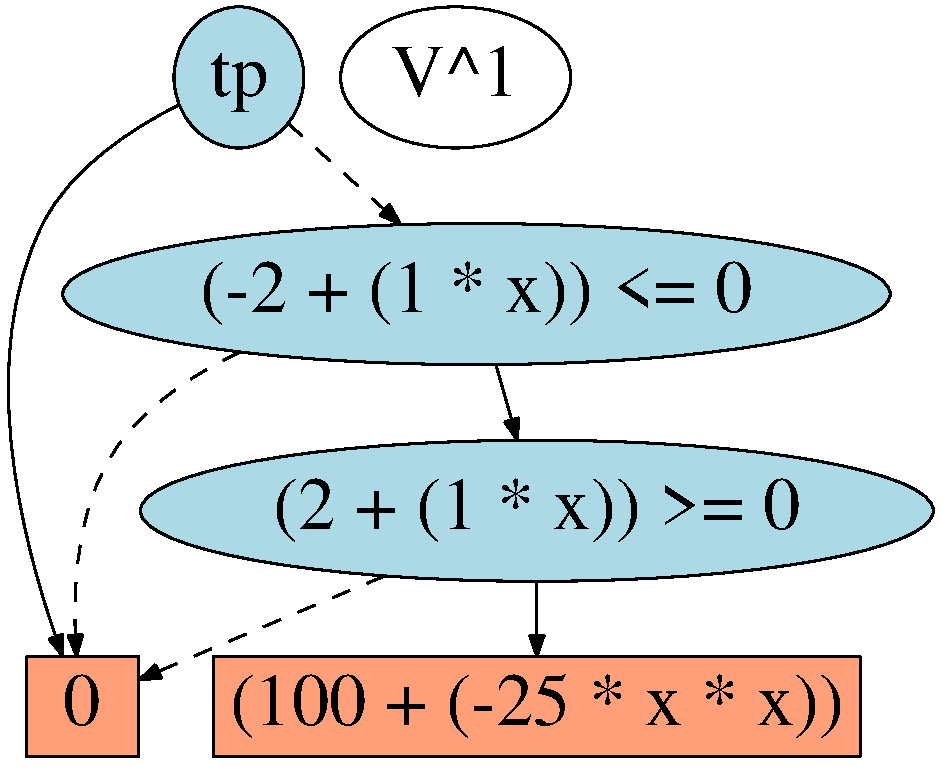
\includegraphics[width=0.33\textwidth]{Figures1/roverR.pdf}
\end{center}
\vspace{-3mm}
\caption{%\footnotesize 
The optimal value function for horizon one of \InventoryControl\ 
as a decision diagram: 
the \emph{true} branch is solid, the \emph{false}
branch is dashed.} \label{fig:rover_R}
\vspace{-3mm}
\end{figure}
%%%%%%%%%%%%%%%%%%%%%%%%%%%%%%%%%%%%%%%%%%%%%%%%%%%%%%%%%%%%%%%%%%%%%%%%%% 

In an XADD the decision nodes can have arbitrary inequalities (one
per node) and the leaf nodes can represent arbitrary functions.
Standard ADD operations to build a canonical ADD and 
to perform a binary operation on two ADDs applies in the case of XADDs.

It is fairly straightforward for XADDs to support all case operations defined in the previous section. 
Binary operations or restriction is done similar to the ADD case while maximization and substitution 
requires reordering of the decision nodes since the former introduces new nodes and the latter modifies
the decision nodes. 

For the maximization of continuous variables, we consider two separate XADDs for the 
upper and lower bounds on the continuous action and then apply the maximum on these two functions. 
This operation is shown in detail in the next section. 

In general, the fact that the decision nodes have internal structure is irrelevant, but means that certain 
paths in the XADD may be inconsistent or infeasible (due to parent decisions).  To further simplify our settings, 
when the XADD has only linear decision nodes, we can use the feasibility checkers of a linear programming solver 
to prune unreachable nodes in the XADD following the approach of []. Using the XADD structure the value
iteration algorithm can scale to much longer horizons compared to the original SDP algorithm. In the next section we introduce the model we use for our SDP algorithm.

\section{Discrete and Continuous State-Action MDPs}

% I have defined action to be continuous only
We assume that a general class of fully observable Markov decision processes with discrete and continuous states and actions can model our domain problems.
The state space is represented by a vector $(\vec{b},\vec{x}) = ( b_1,\ldots,b_n,x_{1},\ldots,x_m )$ consisting of Boolean variables
 $b_i$ ($1 \leq i \leq n$) such that $b_i \in \{ 0,1 \}$ and continuous Real variables $x_j$ ($1 \leq j \leq m$) s.t. $x_j \in [L_j,U_j]$ and $L_j,U_j \in
\mathbb{R}; L_j \leq U_j$.  The action space contains a finite number of continuous actions $A
= \{ a_1, \ldots, a_p \}$ where each $a_{\Delta} \in [L_{\Delta},U_{\Delta}]$ and $L_{\Delta},U_{\Delta} \in
\mathbb{R}; L_{\Delta} \leq U_{\Delta}$.

The transition function is defined as the probability of the next state given the current state and action assuming the Markov property.  Considering the Dynamic Bayesian Network model for modelling each state variable and disallowing synchronic arcs in between them,  results in the following definition for the transition function:   
\begin{align}
P(\vec{b}',&\vec{x}'|\vec{b},\vec{x},a_{\Delta}) = \label{eq:dbn} \\
& \prod_{i=1}^n P(b_i'|\vec{b},\vec{x},a_{\Delta}) \prod_{j=1}^m P(x_j'|\vec{b},\vec{b}',\vec{x},a_{\Delta}) \nonumber 
\end{align}

Here the first probability for binary discrete variables can be represented by conditional probability tables (CPTs). The second probability for continuous variables is represented using conditional stochastic equations (CSEs) wthat are Markovian and deterministic with the definition of any arbitrary (e.g. non-linear) function with continuous actions and states such as:
\vspace{-3mm}
{\footnotesize
\begin{align}
P(x_1' | \vec{b},\vec{b}',\vec{x},a_{\Delta}) = \delta\left[ x_1' - 
\begin{cases}
b_1' \land a_{\Delta} \leq 1 : & \exp(x_1^2 - x_2^2) \\
\neg b_1' \lor  x_2^2 > 1 : & x_1 + x_2 +a_{\Delta} \\
\end{cases}
\right] \label{eq:ex_csde}
\end{align}}
Using the Dirac function the conditional probability is guaranteed to integrate to 1 over the variable, furthermore the probability is stochastic since it conditions on Boolean random variables as well as sampling them stochastically at the same time. \\
The reward function represents the immediate reward of taking an action in a state and it can take the form of any arbitrary function such as:
\begin{align}
R_{a_{\Delta}}(\vec{b},\vec{x}) = \begin{cases}
x_1^2 + x_2^2 \leq 1 : & 1 - x_1^2 - x_2^2  \\
x_1^2 + x_2^2 > 1 : & 2 * a_{\Delta}^2 \\
\end{cases} \label{eq:simple_reward}
\end{align}
The policy $\pi$ specifies which action $a_{\Delta}$ to take in the current state  $(\vec{b},\vec{x})$ and the goal is to find an optimal sequence of policies
$\Pi^* = (\pi^{*,1},\ldots,\pi^{*,H})$ that maximizes the expected sum of discounted reward over a horizon $h \in H $: \\
\begin{align}
V^{\Pi^*}(\vec{x}) & = E_{\Pi^*} \left[ \sum_{h=0}^{H} \gamma^h \cdot r^h \Big| \vec{b}_0,\vec{x}_0 \right], \label{eq:vfun_def}
\end{align}
where $\gamma$ is the discount factor between 0 and 1, and  $r^h$ is the reward in horizon $h$ assuming the state state is at $h=0$.\\
This optimal policy can be obtained using the value iteration algorithm. Starting  with an initial value function, the value of taking an action in the current state is defined using the Q-function:  

\vspace{-3mm}

{\footnotesize
\begin{align}
& Q_{a_{\Delta}^{h+1}}(\vec{b},\vec{x}) = R_{a_{\Delta}}(\vec{b},\vec{x}) + \gamma \cdot \\ 
& \sum_{\vec{b}'} \int_{\vec{x}'} \left( \prod_{i=1}^n P(b_i'|\vec{b},\vec{x},a_{\Delta}) \prod_{j=1}^m P(x_j'|\vec{b},\vec{b}',\vec{x},a_{\Delta}) \right) V^h(\vec{b}',\vec{x}') d\vec{x}' \nonumber
\end{align}
}

Now given the Q-function for each action, the h+1-stage-to-go value function is defined as (3): 
\begin{align}
V^{h+1}(\vec{b},\vec{x}) & = \max_{a \in A} \left\{ Q^{h+1}_a(\vec{b},\vec{x}) \right\} \label{eq:vfun}
\end{align}

If the horizon is finite then the optimal value function continues to the last horizon but if the problem has infinite horizon then a termination criteria is defined, in most problems if the value function of two successive iterations are equal, the algorithm terminates. In the next section we define the symbolic dynamic programming algorithm as the solution to DCA-MDPs.

\section{Symbolic Dynamic Programming (SDP)}

In this section we present our exact algorithm for obtaining the optimal policy for continuous action and states. This algorithm avoids approximating as well as enumerating the state and action. The Continuous state-action dynamic programming (CSA-DP) algorithm in Algorithm 1, implements value iteration for DCA-MDPs producing a sequence of value functions $V^0,V^1,...$ until convergence and uses the XADD structure to efficiently represent state-action partitions.

%%%%%%%%%%%%%%%%%%%%%%%%%%%%%%%%%%%%%%%%%%%%%%%%%%%%%%%%%%%%%%%%%
\incmargin{1em}
%\linesnumbered
\begin{algorithm}[t!]
\SetKwFunction{getCanonicalNode}{{\sc GetCanonicalNode}}
\SetKwFunction{reduce}{{\sc Reorder}}

%\SetKwInOut{Input}{input}
%\SetKwInOut{Output}{output}

%\Input{$F$ (DCA-MDP: discrete-continuous states, continuous actions, transition and reward function)}
%\Output{$F_r$ (Value function $V^h$ and optimal policy $\pi^*$)}
\BlankLine
\Begin{
   \textbf{if} R is action independent \textbf{then} set $V^0=R$     \textbf{else} $V^0 = 0$\\
   \While {$h < \mathit{maxHorizon}$}{
      	\ForEach { action variable $\Delta$ in A }{
      		Prime Value-function($V^{'h}$)using substitute\\
      		\ForEach {continuous state variable in S}
      		
      		{
      			Perform Continuous integration: 
      			\begin{align}
      			\tilde{Q}_{a_{\Delta}^{h+1}} :=\int_{x_j'} \delta[x_j' - g(\vec{x})] V'^{h} dx_j' \; \\
      			      			= \; V'^{h} \{x_j' / g(\vec{x}) \}
      			\end{align}
      		}
      		
      		\ForEach {discrete state variable in S }
      		
      		{
      			Perform Discrete marginalization: 
      			\begin{align}
      			\tilde Q_{a_{\Delta}^{h+1}} := \left[\tilde Q_{a_{\Delta}^{h+1}} \otimes P(b_i'|\vec{b},\vec{x},a) \right]|_{b_i' = 1} \nonumber \\
      		   	 \oplus \left[\tilde Q_{a_{\Delta}^{h+1}} \otimes P(b_i'|\vec{b},\vec{x},a) \right]|_{b_i' = 0}
      		   	\end{align}
      		}
      		Multiply discount factor $\gamma$
      		\begin{align*}
      		\tilde Q_{a_{\Delta}^{h+1}} = \tilde Q_{a_{\Delta}^{h+1}} \otimes \gamma
      		\end{align*}
      		Add Reward function to Q-function:
      		\begin{align*}
      		\tilde Q_{a_{\Delta}^{h+1}} = \tilde Q_{a_{\Delta}^{h+1}} \oplus R
      		\end{align*}
      		
      		\ForEach {case partition in $\tilde Q_{a_{\Delta}^{h+1}}$ }
      		{
      			 1- Compute bounds on $\Delta$: (UB, LB, Roots)
      			
      			 2- Evaluate $\tilde Q_{a_{\Delta}^{h+1}}$ using bounds
      			(Substitute and take maximum)
      			
      			 3- Add bound constraints ()$LB\leq Roots\leq UB$) 
      		}
      	}
      	
      	Compute new Value function: 
      	\begin{align}
      	V^{h+1} & = 
      	\max(Q_{a_1}^{h+1},\max(\ldots,\max(Q_{a_{p-1}}^{h+1},Q_{a_p}^{h+1})))
      	\end{align}
      }
}
\caption{{\sc CSA-DP} }
\end{algorithm}
\decmargin{1em}
%%%%%%%%%%%%%%%%%%%%%%%%%%%%%%%%%%%%%%%%%%%%%%%%%%%%%%%%%%%%%%%%%

We now describe each section of the algorithm using the \MarsRoverNL example. 

\begin{enumerate}
\item The symbolic value iteration algorithm works with the XADD structure for efficiency. This means that each of the i-stage-to-go value functions ($V^i$) is set to be an XADD. In most problems in this domain, the reward function defines action costs as a penalty to avoid the agent of acting more than required. For this reason we define the first value function equal to zero $V^0=0$ which is a tree with only one leaf node [0]. If the reward function of the DCA-MDP is independent of the actions, then the first value function can be equal to this reward $V^0=R$.\\

\item Next, for $h > 0$ the algorithm iterates over the horizon until a convergence criteria is met or in our case the maximum number of iterations is reached. The next parts of the algorithm is performed for each horizon. For each horizon we take a continuous action $\Delta$ and perform the following steps in sequence.\\

\item The first step of value iteration for horizon $h$, action $\Delta$ is to prime the current state so it becomes the next state. This can be performed by substituting the state variables with their primed versions. Given as an example in section 2 , we set
{\footnotesize
\begin{align*}
\sigma = \{ b_1 / b_1', \ldots, b_n / b_n', x_1 / x_1', \ldots, x_m / x_m' \}
\end{align*}
}
and obtain $V'^{h} = V^{h}\sigma$.

\item Next, we need to consider the back-up step of the Bellman equation of ~\eqref{eq:qfun} restated here: 
 \vspace{-3mm}
 
 {\footnotesize
 \begin{align}
 & Q_a^{h+1}(\vec{b},\vec{x}) = R_a(\vec{b},\vec{x}) + \gamma \cdot \label{eq:qfun} \\ 
 & \sum_{\vec{b}'} \int_{\vec{x}'} \left( \prod_{i=1}^n P(b_i'|\vec{b},\vec{x},a) \prod_{j=1}^m P(x_j'|\vec{b},\vec{b}',\vec{x},a) \right) V^h(\vec{b}',\vec{x}') d\vec{x}' \nonumber
 \end{align}}
 
We first evaluate the integral marginalization $\int_{\vec{x}'}$ over the continuous variables in the algorithm. For each of the continuous variables $x'_j$, the only functions dependent on this variable are $V'^{h}$
and $P(x_j'|\vec{b},\vec{b}',\vec{x},a) = \delta[x_j' - g(\vec{x})]$; 
hence, marginal over $x_j'$ need only be computed over
their product. Also according to [] this integration is equal to substituting $\sigma = \{ x_j' / g(\vec{x}) \}$
on $V'^{h}$ as shown in (11) and (12) in the algorithm.

This substitution is performed for each $x_j'$ ($1 \leq j \leq m$) updating $\tilde{Q}_a^{h+1}$ each time,
then after elimination of all $x_j'$ the partial regression of $V'^{h}$ for the continuous variables for
each action $a$ is denoted by $\tilde{Q}_a^{h+1}$. Substitution preserves the disjoint partition property, so given that the previous value function is also a case statement, substituting it with the transition function which is again in the form of a case statement, produces $\tilde{Q}_a^{h+1}$ as a case statement that can also be presented by an XADD.
% need to mention conditional substitution here??? 

\item The next step is to complete the backup step using $\tilde{Q}_a^{h+1}$. 
For this we consider marginalization of discrete variables $\sum_{\vec{d}'}$ in~\eqref{eq:qfun}.
The discrete regression applies the following iterative process for each $d_i'$ according to (13).
As explained in an example for the restriction operator $|_v$ the variable v is set to the given value if present.
Both $Q_a^{h+1}$ and $P(b_i'|\vec{b},\vec{x},a)$ are represented
as case statements and restriction preserves this property, thus after marginalizing over all $\vec{b}'$ , the resulting $ \tilde{Q_a^{h+1}}$ is the symbolic representation
of the intended Q-function.


\item Now that we have $Q_a^{h+1}$ in
the case format we perform continuous maximization for action $\Delta$ as explained in section (2.1). Figure 2 also explains this step visually using XADDs from the \MarsRoverNL problem. We take each case statement which are disjoint partitions on the state-action space independently and keep a running maximum for the result. In Figure 2, we shown 2 of the ??  branches and consider the steps of our algorithm on them.
For each such partition, we first build the bounds on $\Delta$ based on the nodes: 
\begin{enumerate}
\item Consider two XADDs for the UB, LB and the root
\item For each decision node , isolate the action $\Delta$ variable on the LHS and take everything to the RHS.
\item Divide the RHS by the coefficent of $\Delta$
\item Flip the inequality sign if the false branch of the parent decision is considered or the coefficient of $\Delta$ is negative. 
\item Consider the RHS as the UB if inequality is ($<, \leq$), else add RHS to the LB.
\item Perform Symbolic Minimum on the upper bound XADD and Symbolic Maximum on the lower bounds
\item Take first derivative of the Leaf of this case partition and equal that to zero
\item If a value (constant or variable) appears for action $\Delta$ this is the root value.(XADD with single node)
\item The two resulting XADDs now have the UB, LB and roots for this branch
\end{enumerate}


Figure 2 shows the XADDs for the UB,LB and root. Having obtained the XADDs for the bounds, we now evaluate the bounds on the Q-function value at the leaf. This is equal to substituting the bounds in the leaf for $\Delta$.
% add substitute formula? done it before

We then take the maximum of the bounds with regard to the new XADDs. This is equal to the Symbolic maximum over three different functions which is an XADD itself: 
% add maximum function?already done it with examples

In the last step, we add the constaints for the bounds as well as the action-independent decisions of this partition to the resulting XADD. Figure 2 shows the end result XADD for both partitions. The running maximum which is an initially empty XADD is now used to take the maximum of each branch after they are produced. By the time all the case statements of $ \tilde{Q_a^{h+1}}$ have been processed in this algorithm, the running maximum will contain the maximum over all the partitions which is independent of action $\Delta$ now, or the  $V_{\Delta}^{h+1}$

This algorithm is performed for each of the continuous actions in $a \in \{a_1,\ldots,a_p\}$ separately. Obtaining the overall $V^{h+1}$ in case format as defined in ~\eqref{eq:vfun} requires sequentially applying \emph{symbolic maximization} as defined in (14).
\end{enumerate}

We illustrate the maximization algorithm using the \MarsRoverNL example in Figure ~\ref{fig:rover_algorithm}. The non-linear branch of the value function of iteration one is illustrated as in section 2.1. 
The other branches follow the algorithm to obtain the final result of Figure ~\ref{fig:rover_V2}. The pruning approach of [] is used to prune the branches as well as a linearization approach. In this method we take all non-linear decision nodes and convert them into their equivalent linear nodes. As an example of the \MarsRoverNL we have the following:

{\footnotesize 
\begin{center}
\begin{tabular}{r c c c l}
&
$\begin{cases}
(96.4 + x^2 -20*x>=0): 0 \\ 
\neg(96.4 + x^2 -20*x): -2410 - 500*x - 25*x^2\\ 
  \end{cases}$
\\ \\
&
  $\begin{cases}
(-11.897366596101026 + (1 * x) >= 0): 0\\ 
(-8.102633403898974 + (1 * x) <= 0) \wedge \\
\neg(-11.897366596101026 + (1 * x) >= 0):0\\ 
(-8.102633403898974 + (1 * x) >= 0) \wedge \\
\neg(-11.897366596101026 + (1 * x)<= 0):\\
 -2410 - 500*x - 25*x^2\\ 
  \end{cases}$
\end{tabular}
\end{center}
}
%%%%%%%%%%%%%%%%%%%%%%%%%%%%%%%%%%%%%%%%%%%%%%%%%%%%%%%%%%%%%%%%%%%%%%%%%%
% CSA-DP sketch of algorithm using marsrover example
\begin{figure*}[t]
\begin{center}
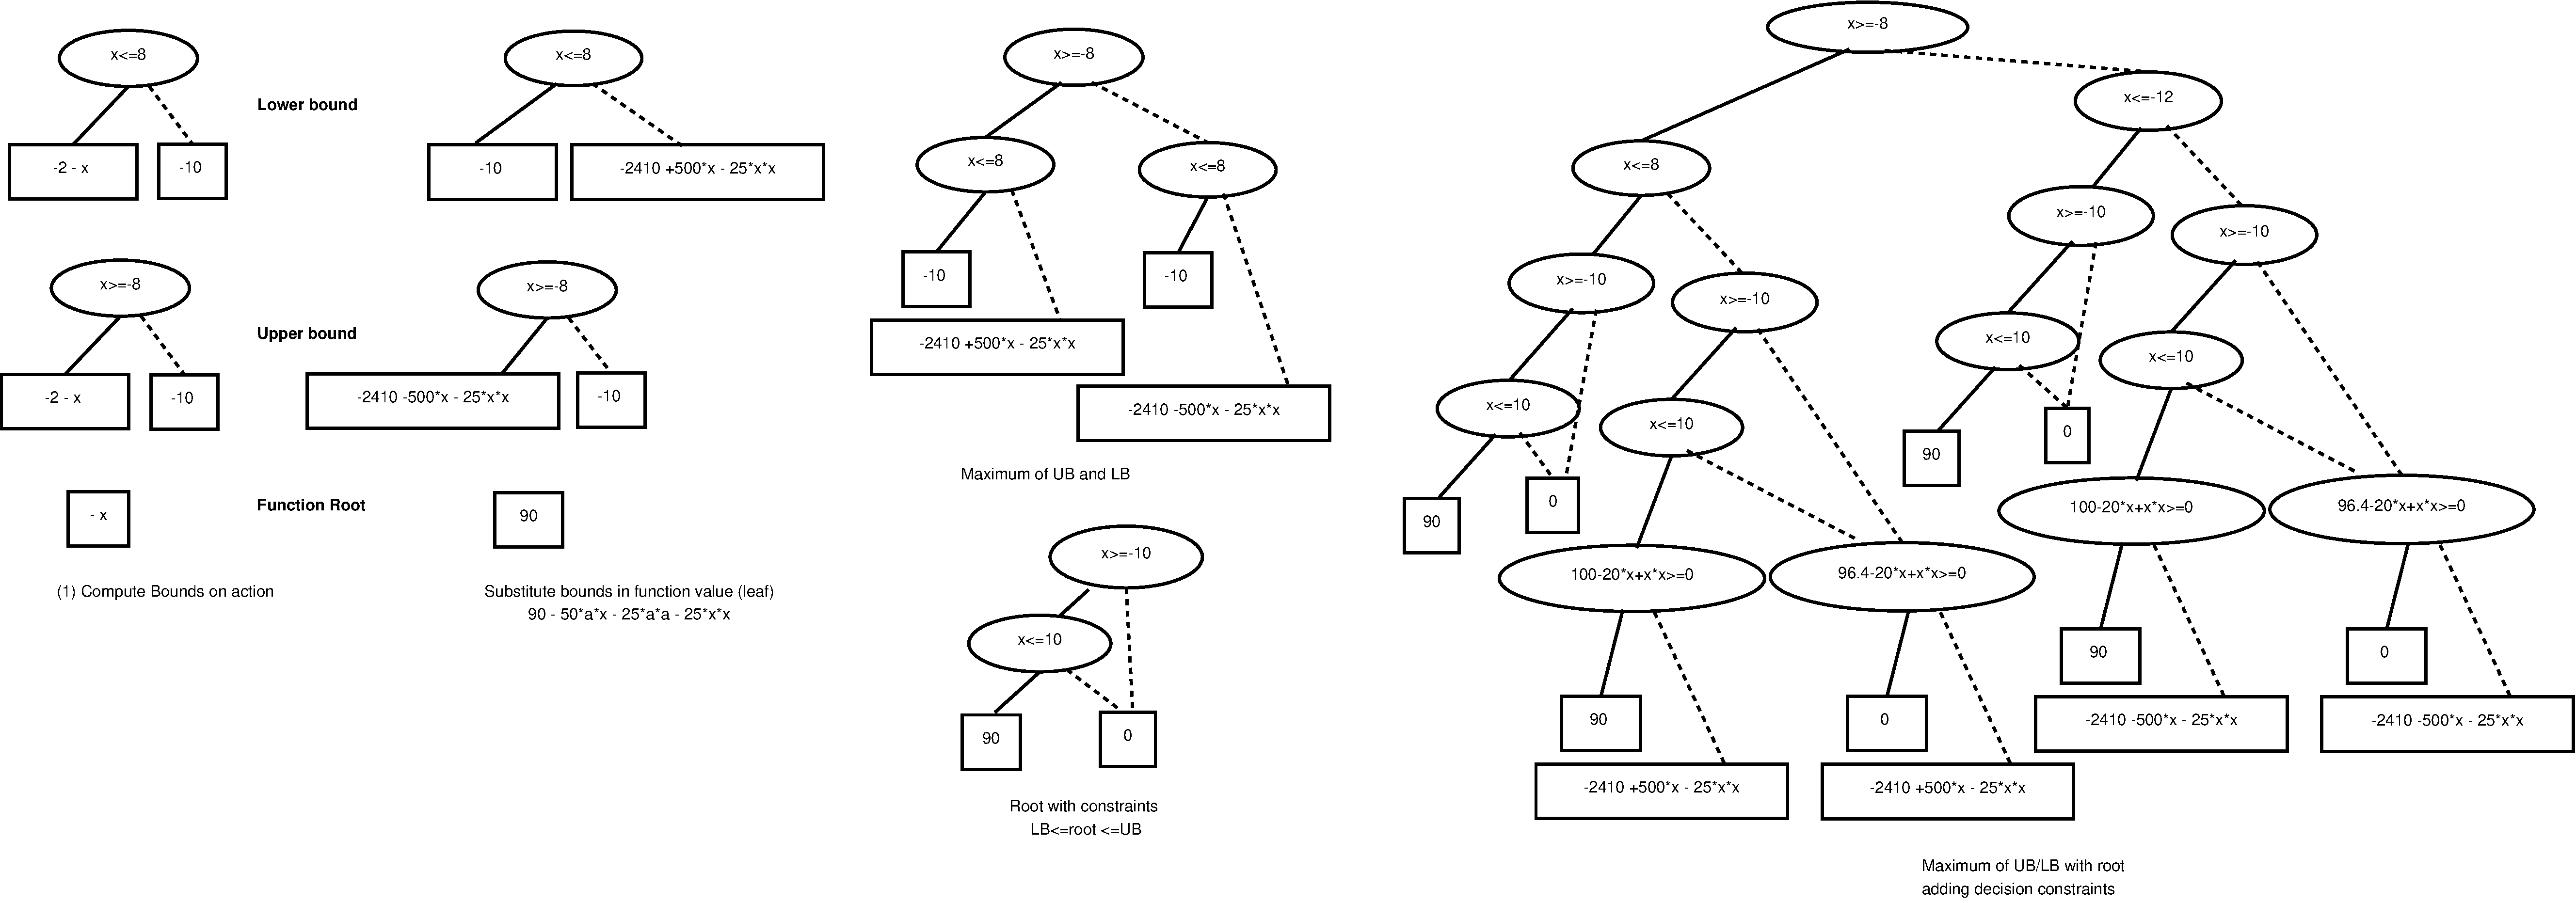
\includegraphics[width=0.7\textwidth]{Figures1/maximum_cont_action.pdf}
\end{center}
\vspace{-3mm}
\caption{%\footnotesize 
Continuous maximization in CSA-DP using one branch of \MarsRoverNL example\
} \label{fig:rover_algorithm}
\vspace{-3mm}
\end{figure*}
%%%%%%%%%%%%%%%%%%%%%%%%%%%%%%%%%%%%%%%%%%%%%%%%%%%%%%%%%%%%%%%%%%%%%%%%%%
%%%%%%%%%%%%%%%%%%%%%%%%%%%%%%%%%%%%%%%%%%%%%%%%%%%%%%%%%%%%%%%%%%%%%%%%%%
% V2 for marsrover
\begin{figure*}[t]
\begin{center}
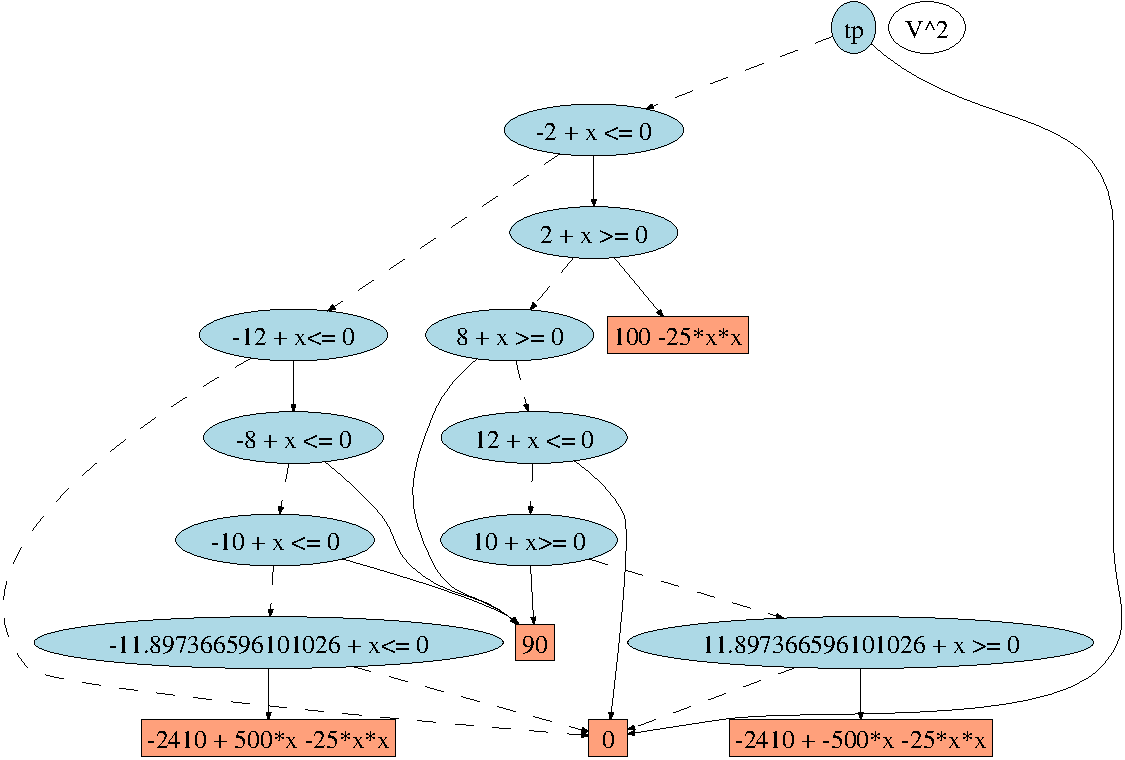
\includegraphics[width=0.3\textwidth]{Figures1/v2.pdf}
\end{center}
\vspace{-3mm}
\caption{%\footnotesize 
The final value function for the second horizon of the \MarsRoverNL example\
} \label{fig:rover_V2}
\vspace{-3mm}
\end{figure*}
%%%%%%%%%%%%%%%%%%%%%%%%%%%%%%%%%%%%%%%%%%%%%%%%%%%%%%%%%%%%%%%%%%%%%%%%%%



\section{Empirical Results}

We implemented the CSA-DP algorithm using the XADDs and tested it on several domains. The first which has been used as the example throughout the paper is the \MarsRoverNL, also we have two problems from the OR literature; \InventoryControl and \WaterReservoir. We give the empirical results for these domains next.
\subsection{\MarsRoverNL}
The problem specifications and some parts of the solution have already been presented in the previous sections. Here we take a closer look at the exact value function for three different horizons. 

This plot visualizes non-linear piecewise boundaries which occurs due to non-linear leaves in the XADD ;equivalent to non-linear partitions of the state space. It shows that the Rover can move non-linearly (quadratic) around the target radius (i.e, [-2,2]) progressively to get to the exact point with high precision. It then achieves a constant optimal value after the radius and before reaching the action boundaries in each iteration (i.e, the rover can move at most between [-10,10] in each iteration). After the boundaries the rover moves according to a non-linear function thus achieving a non-linear value which was demonstrated in Figure~\ref{fig:rover}. 

Every step of the algorithm allows the Rover to move from further distances towards the radius, hence the constant step and the non-linear curvature at the boundaries occur iteratively. This example clearly demonstrated the power of the CSA-DP algorithm for non-linear functions.

We note that these results were generated  with the XADD pruning which consists of linear pruning using the LP solver and non-linear pruning using the linearization method.
Without the pruning, even in low horizons, because of infeasible branches, time and space grows exponentially. We have also used the general pruning method of XADDs as in [] for the other domain problems.
%%%%%%%%%%%%%%%%%%%%%%%%%%%%%%%%%%%%%%%%%%%%%%%%%%%%%%%%%%%%%%%%%%%%%%%%%%
% 2d plots for mars rover to show non-linear movements
\begin{figure*}[t]
\begin{center}
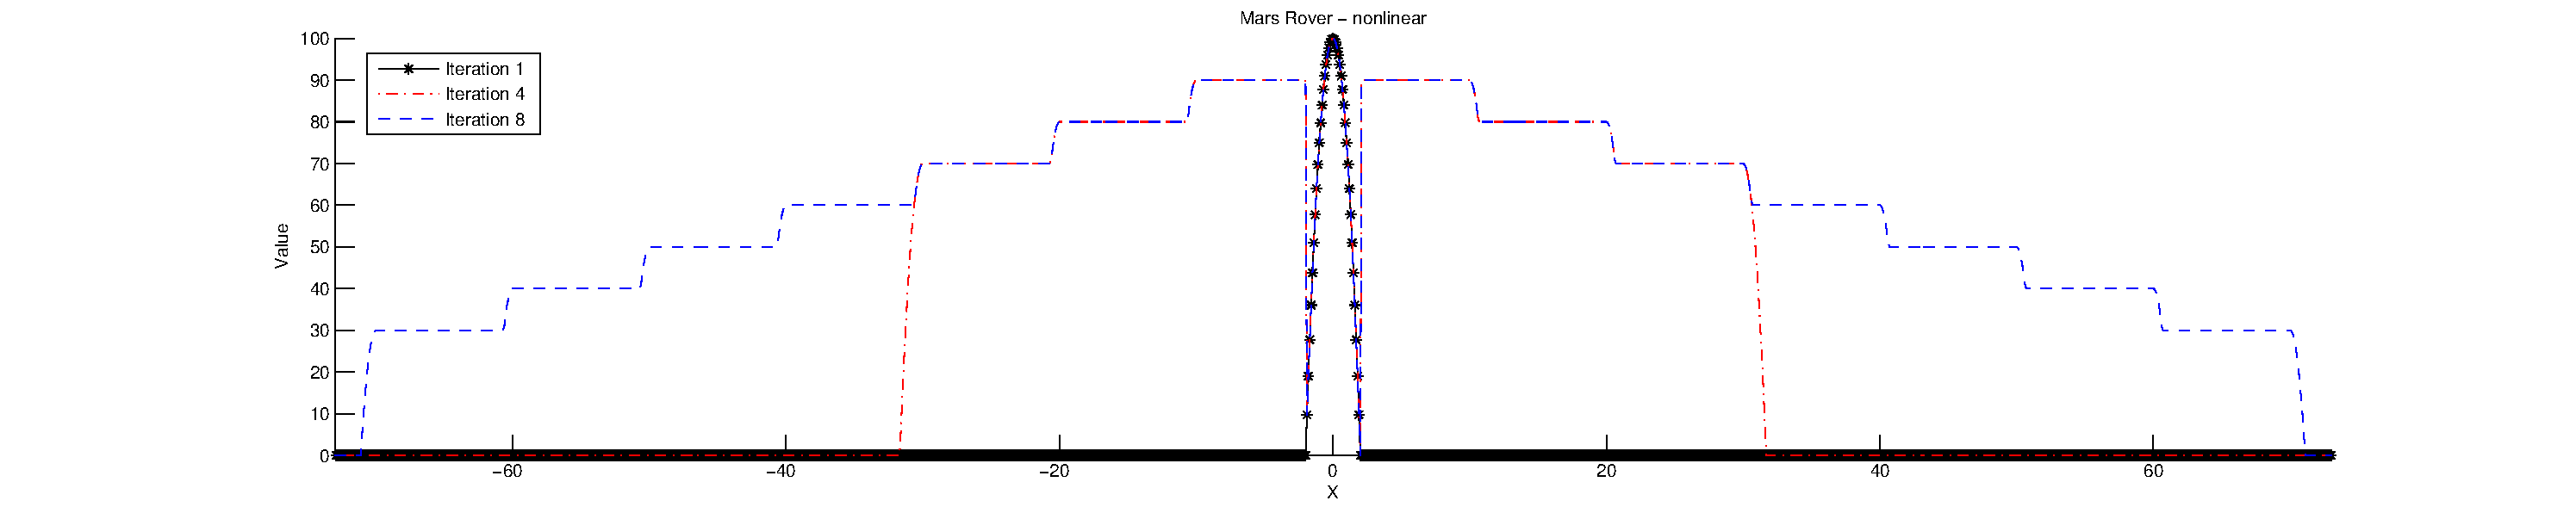
\includegraphics[width=0.37\textwidth]{Figures1/rover.pdf}
\end{center}
\vspace{-3mm}
\caption{%\footnotesize 
The optimal value function for horizon 1-4-8 of \MarsRoverNL\ 
} \label{fig:rover}
\vspace{-3mm}
\end{figure*}
%%%%%%%%%%%%%%%%%%%%%%%%%%%%%%%%%%%%%%%%%%%%%%%%%%%%%%%%%%%%%%%%%%%%%%%%%%
\subsection{\InventoryControl} 
This domain problem has become a benchmark problem for optimization in the OR literature and applies to our general DCA-MDP setting. Business firms often deal with the problem of deciding  the amount of product to order in a time period such that customer demands are satisfied. The firm's warehouse will keep an inventory of this product to deal with different customer demand levels. Each month, the firm must decide on the amount of products to order based on the current stock level.
The order should not be too high since keeping the inventory is expensive, nor should it be too low in which case it will be penalized for being unable to meet customer demands and leading to loss of customers. The optimization problem faced by the firm is to find an optimal order policy that maximizes the profit.

We present a simple formulation of this problem where the capacity of the inventory is C units of each product and customer orders not satisfied in this month are backlogged for the next month, so inventory can take negative values. We consider two cases, a one product inventory with one order action and the other with two products that needs two different orders.

We take two continuous state variable $x_1,x_2 \in [-1000,C]$ indicating the current inventory quantity into account, with the total inventory capacity of 800, and a stochastic boolean state variable for customer demand level $d$ where $d=0$ is low demand levels (50) and $d=1$ is high demand levels (150) according to some probability. \\
The continuous action variable is the order quantity $a_1,a_2 \in [0,C]$ which can at most take the value of the maximum inventory capacity. \\

We define an immediate negative reward for the cost of producing an order and the storage cost of holding the products in the inventory and also a positive reward for fulfilling the customer demand whenever there are enough stocks in the inventory. The transition for one of the state variables and reward function are defined below:
%\ because of backlogging, the customer demand is always taken from the current stock level, leaving it negative
%\ consider the next state as the current state and orders minus the customer orders
%\ customer demands are boolean of low and high that change in every iteration
%\ 

{\footnotesize
\begin{align*}
x'_1 & = \begin{cases}
d  \wedge (x_1 + a_1 + x_2 - 150 \leq 800) : & x_1 + a_1 - 150 \\
d  \wedge (x_1 + a_1 + x_2 - 150 \geq 800) : & x_1 - 150  \\
\neg d \wedge (x_1 + a_1 + x_2 - 150 \leq 800): & x_1 + a_1 - 50    \\
\neg d \wedge (x_1 + a_1 + x_2 - 150 \geq 800): & x_1 - 50    \\
\end{cases}\\
d' & =  \begin{cases}
d     : &(0.7)\\
\neg d: &(0.3)\\
\end{cases}\\
R & = \begin{cases}
(x_1 + x_2 \geq 900) \wedge d\\
150 - 0.5\cdot a_1 -0.4 \cdot a_2 - 0.1\cdot(x_1 + x_2) \\
(x_1 + x_2 \leq 900) \wedge d\\
(150 - (x_1+x_2)) - 0.5\cdot a_1 -0.4 \cdot a_2 - 0.1\cdot(x_1 + x_2) \\
(x_1 + x_2 \geq 300) \wedge \neg d\\
50 - 0.5\cdot a_1 -0.4 \cdot a_2 - 0.1\cdot(x_1 + x_2) \\
(x_1 + x_2 \leq 300) \wedge \neg d\\
(50 - (x_1+x_2)) - 0.5\cdot a_1 -0.4 \cdot a_2 - 0.1\cdot(x_1 + x_2) \\
\end{cases}
\end{align*}}

% write description in case we have to take this huge case out! 
The transition for the continuous actions partitions based on the maximum capacity of the inventory (for both products), and only adds the orders if the current total capacity (with respect to the orders of that product and the stocks available for both products) are less than this maximum capacity. 

The demand variable is transitioned stochastically and the reward function is based on the demand levels and the current stock in inventory. If the current stock is larger than the total inventory, we get the reward for fulfilling the demand $(e.g 150)$, if the demand is high and the inventory is not high enough, then the reward is $(e.g (150 - (x_1+x_2)))$, in both cases the action costs and holding costs are also added. This allows the inventory to stock as many products as possible while not exceeding the capacity of the inventory. 

We plot the results of comparing a 1-product \InventoryControl problem with a multi-dimensional one. Figure~\ref{fig:invC} compares the time and nodes for different iterations for these two problem instances and a third comparisoon for the effect of not pruning on the 1D instance. This demonstrates the impact of having multiple constraints and action variables on the problem size which requires much more state-action partitions. The time and space have increased from the first iteration up to the third iteration for the 2D problem size, but then dropped for the next horizons due to pruning the XADD in our algorithm. As more constraints got added in for horizon 4, they cancelled the effects of some of the previous branches because of infeasibility and the pruning operation allows the XADD to grow smaller in space and requiring almost a constant time depending on the constraints added in each horizon. Without considering pruning, even the 1 product problem instance quickly falls into the curse of dimensionality problem and as the figure shows, time and space grow non-linearly after the second iteration. 
% any need for 3d plot? For the 1 or 2 product case?
% any thing else we need from this example?
%%%%%%%%%%%%%%%%%%%%%%%%%%%%%%%%%%%%%%%%%%%%%%%%%%%%%%%%%%%%%%%%%%%%%%%%%%
%figure5 : time-iteration and space-iteraton for 1d-2d-noPrune inventory
\begin{figure*}[t]
\centering
%\subfigure{
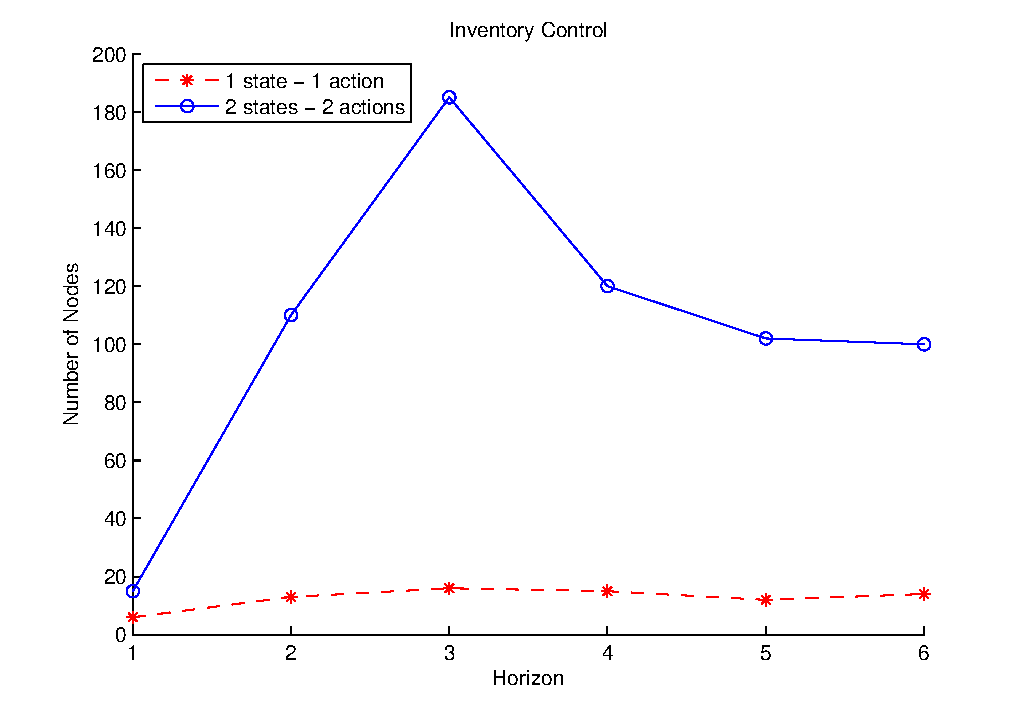
\includegraphics[width=0.4\textwidth]{Figures1/space1-2.pdf}
\hspace{5mm}
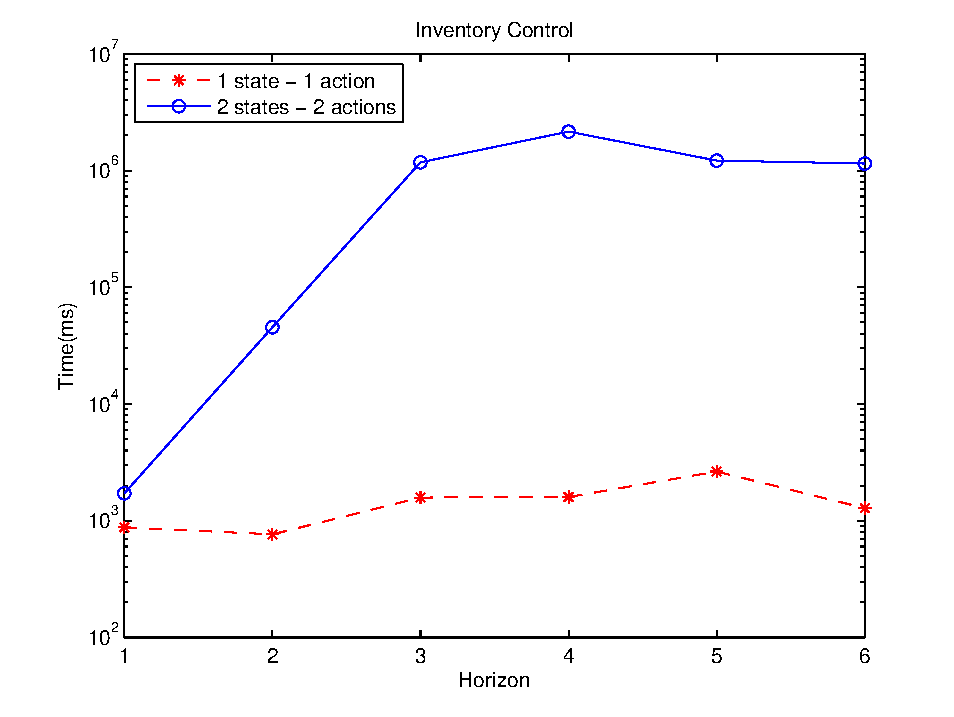
\includegraphics[width=0.4\textwidth]{Figures1/time1-2.pdf}
%}
%\vspace{-3mm}
\caption{%\footnotesize 
Space (\# XADD nodes in value function) and
time for different horizons of CSA-DP on \InventoryControl\ 
Comparing 1D, 2D and no-pruning}
\label{fig:invC}
%\vspace{-3mm}
\end{figure*}
%%%%%%%%%%%%%%%%%%%%%%%%%%%%%%%%%%%%%%%%%%%%%%%%%%%%%%%%%%%%%%%%%%%%%%%%%%


\subsection{\WaterReservoir}The problem of \WaterReservoir needs to make an optimal decision on how much and when to discharge water from water reservoirs to maximize hydroelectric energy productions while considering environment constraints such as irrigation requirements and flood prevention. 
A multi-reservoir system is more desirable than the single reservoir problem due to its ability in controlling various environment parameters such as flooding.  In these systems, the inflow of downstream reservoirs are effected by the outflow of their upstream reservoirs. In the OR literature, this case  is considered much more complex and for the sake of simplicity mainly the single case in considered. For multi-reservoirs the main problem that leads to approximations to DP methods or using other simplifications is the curse of dimensionality. In this domain the discharge action is considered as a discrete action  and so are the energy demands. This causes the state space to grow exponentially in case of multiple states and actions[].
Using our method for continuous action value iteration, we show that this problem can be handled efficiently and is scalable to multi-reservoir problems. Consider a two-level reservoir with the outflow of the second reservoir added to the input of the first reservoir. The state space is the level of water in both reservoirs as well as the energy demands and inflow (such as rainfall or streams) to the reservoirs $(l1,l2,i,e)$. We consider the water levels as continuous variables, the inflows to both reservoirs are the same which depends on a high-low sessions of rainfall. The energy demands e can be considered both continuous or discrete for different customer needs. 

We want to prevent the upstream reservoir ($l2$) from reaching low water levels, while avoiding flooding which is caused by high water levels. A constant amount of water is discharged from the downstream reservoir($l1$) to meet customer electricity demands. The inflow to both reservoirs is assumed to be the same (same amount of rainfall) 

The reward is assigned based on preventing the flood. If water levels prevent flooding, a reward is given for the \textit{time} the reservoir selects the action of discharging water from one reservoir to the other($l2 to l1$), or the choice of not discharging at that time, depending on the water levels. The elapsed time is used as the reward value if the constraints are met, in this case the system should choose to perform an action (drain or no drain) as latest as possible. 
This elapsed time is added to the current time at each transition. The water levels are transitioned based on the previous levels and the amount of discharge and inflow multiplied by the elapsed time. This means that higher elapsed time is desired to maximize the reward, while lower ones ensure flood prevention.

In order to demonstrate the effectiveness of planning optimally with our model, we use this continuous-time example of the multi-reservoir where the elapsed time is defined as the action parameter to drain a reservoir. The goal is to show a form of value function refinement that is generated using this CSA-DP algorithm. The optimal value function will obtain higher values for higher horizons, while the value for lower horizons were less than the current value function. This is demonstrated in Figure~\ref{fig:reservoir} where three value functions have been presented in different horizons. 

Here flood prevention is ensured in each step by the linear piecewise boundaries on the very high and very low levels, the action of discharging occurs here either at time 0 for very critical points or at a time depending on the water levels later during the iteration (i.e, $a = -8.18 + 0.0018*l1$ if one of the water levels is above the critical level in the third iteration). As for the constant section, this piece is the safe range and the action of discharge (or not discharge) is left till the latest possible time thus achieving higher rewards. As the iteration number increases, the future discounted reward goes higher than the previous horizon. 

%%%%%%%%%%%%%%%%%%%%%%%%%%%%%%%%%%%%%%%%%%%%%%%%%%%%%%%%%%%%%%%%%%%%%%%%%%
%figure6 : 3d plots of refinement planning for 3 horizons
\begin{figure*}[t]
\centering
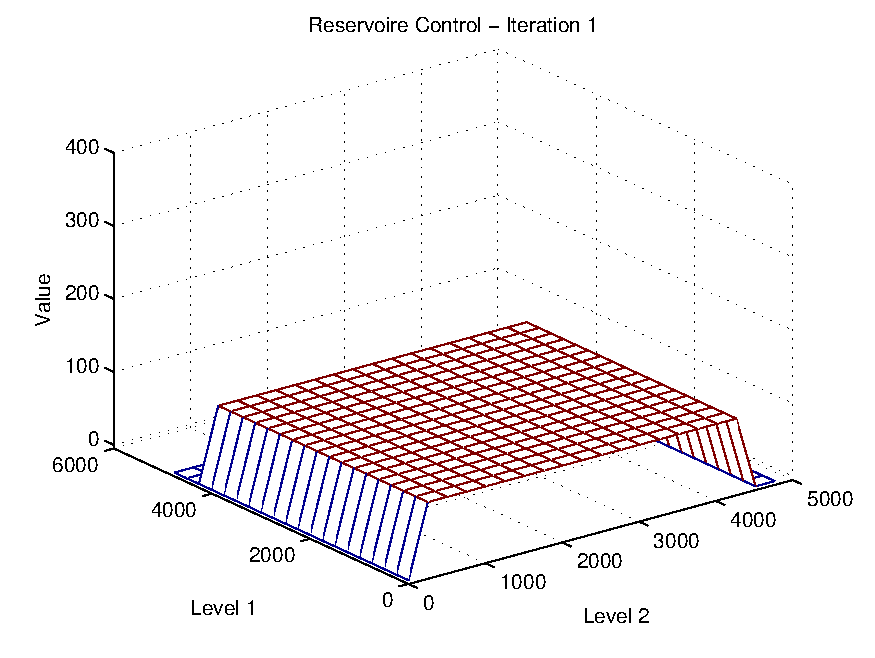
\includegraphics[width=0.33\textwidth]{Figures1/ref1.pdf}
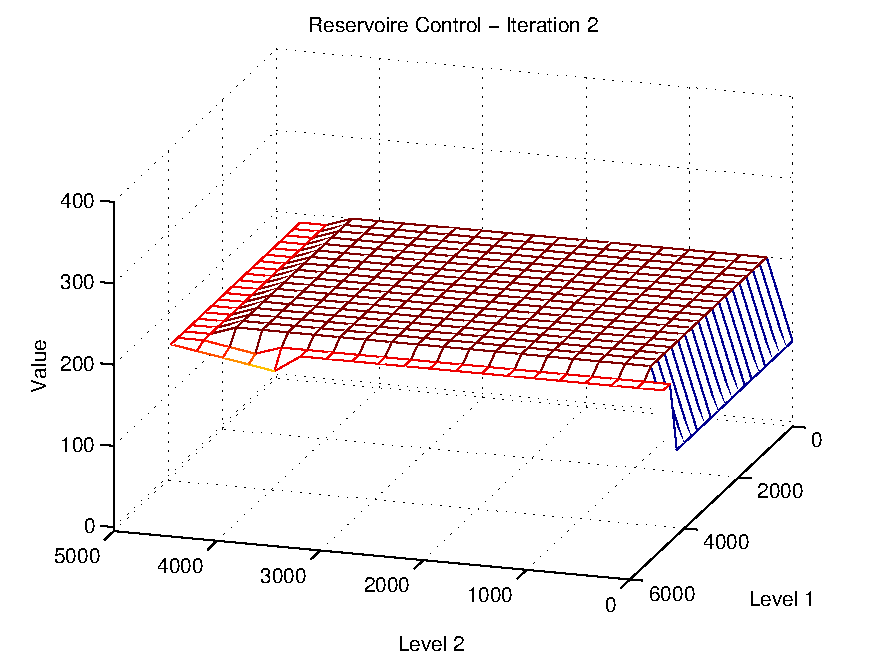
\includegraphics[width=0.33\textwidth]{Figures1/ref3.pdf}
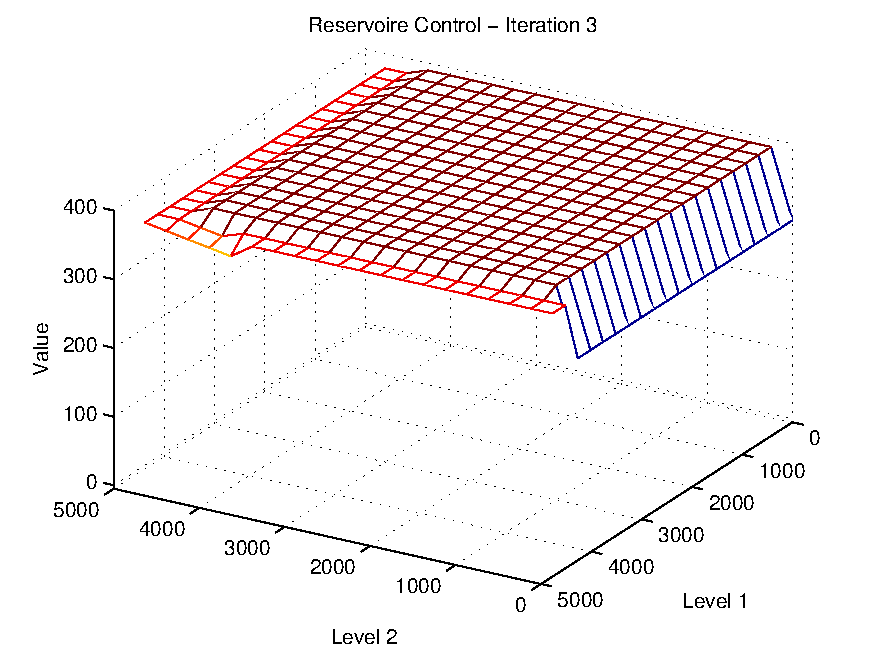
\includegraphics[width=0.33\textwidth]{Figures1/ref6.pdf}
\caption{%\footnotesize 
Exact optimal value function for \WaterReservoir domain
}
\label{fig:reservoir}
%\vspace{-3mm}
\end{figure*}
%%%%%%%%%%%%%%%%%%%%%%%%%%%%%%%%%%%%%%%%%%%%%%%%%%%%%%%%%%%%%%%%%%%%%%%%%%

\section{Related Work}
Markov Decision Processes have been used as the framework of many planning problems that consider uncertainty with continuous resources ~\cite{bresina02}. Many of the previous works have considered continuous state spaces and built exact or approximate Dynamic Programming algorithms to solve the MDP problem. Among these works, the most relevent work to our work is ~\cite{sanner11} which considers solving the MDP for discrete and continuous state variables. 
Here we offer continuous actions such as time or movement for our domain. The theoretical framework of DCA-MDP is similar to ~\cite{Rachelson08} for considering continuous state and action spaces and the mathematical proofs for extending the MDP framework are provided here, but we presented practical application of this framework using XADDs and the CSA-DP algorithm. 

Most work in the continuous action area consider time-dependent models (TMDP) and consider time as a continuous action and solve the MDP problem. In ~\cite{boyan00} time is considered as a continuous variable and the exact solutions exist, but they are limited to the piecewise linear value function setting. 
Sampling ~\cite{Weinstein2010} and approximating ~\cite{pegasus} the continous action space is the most common solution. 

\section{Conclusions}



\section*{Acknowledgements}


\bibliography{action_cont}
\bibliographystyle{aaai}
\end{document}
